% !TEX program = pdflatex
% LTeX: language=en-GB

\documentclass[11pt, a4paper,twosided]{amsart}

  \usepackage[margin=2.5cm]{geometry}
  \usepackage[T1]{fontenc}
  \usepackage[utf8]{inputenc}
  \usepackage{microtype}

% Fontes and co
  \usepackage{newtxtext,newtxmath}
  \usepackage{helvet}
  \usepackage{xcolor}
    \definecolor{Navy}{HTML}{12355B}
    \definecolor{DarkGray}{HTML}{222222}
    \definecolor{LightGray}{HTML}{666666}


\usepackage{url}
\usepackage[normalem]{ulem}
% \usepackage{tablefootnote}
  \usepackage{threeparttable}


% Section Titles
%------------------------------------------------
\color{DarkGray}  

\usepackage[explicit]{titlesec}

\titleformat{\section}
{\Large\sffamily\bfseries\color{Navy}}
{\thesection}
{0.8em}
{#1}
[\vspace{0.3em}\titlerule]

\titleformat{\subsection}
{\large\sffamily\bfseries\color{Navy}}
{\thesubsection}
{0.7em}
{#1 \vspace{-.7em}}

\titlespacing*{\section}
{0pt}{3ex}{1.2ex}

\makeatletter  
  \titleformat{\subsubsection}[runin]
  {\bfseries\normalsize\color{Navy}}
  {\thesubsubsection}{0.7em}{#1}[{\@addpunct{.}}]   
\makeatother
  
  \titlespacing*{\subsection}
  {0pt}{1.8ex}{0.8ex}

  % TOC title
  \usepackage{titletoc}
\renewcommand{\contentsname}{Contents}

\titlecontents{section}
  [0em]
  {\addvspace{0.3em}\sffamily\bfseries\color{Navy}}
  {\contentslabel{2em}}
  {}
  {\hfill\contentspage\vspace{-.3em}}

\titlecontents{subsection}
  [2.2em]
  {\vspace{-.3em}\small}
  {\contentslabel{2.5em}}
  {}
  {\titlerule*[0.5pc]{.}\contentspage}
  [\vspace{-.2em}]
  
  % runnin toc
  \makeatletter
  \titlecontents*{subsubsection}[2.2em]{\vspace{-.2em}\small\parindent=0pt\itshape\relax\S~}{\thecontentslabel\enspace}{}
	{{\@addpunct{,}} p.~\thecontentspage}[ \S ][.]
\makeatother

 % --- paragraph style -----
  \setlength{\parindent}{0pt}
  \setlength{\parskip}{\medskipamount}   
  \usepackage{setspace}
  \setstretch{1.15}

% --- figures and tables --------------
\usepackage{tikz}
  \usetikzlibrary{arrows.meta,decorations.text}
\usepackage{booktabs}
\usepackage{caption}
	\captionsetup[figure]{name=Fig.,font={small}, textfont=it,labelfont=bf,margin=0pt, skip=.5em}	
	\captionsetup[table]{name=Tab.,font={small}, textfont=it,labelfont=bf,margin=0pt, skip=.5em}	
\usepackage{array}

% Headers & Footers
%------------------------------------------------
\usepackage{fancyhdr}
  \usepackage{lastpage}
  \pagestyle{fancy}
    \fancyhf{}

    \fancyhead[LO]{\small\sffamily Fundamental Mathematics in the Age of AI}
    \fancyhead[LE,RO]{\footnotesize\sffamily \thepage/\pageref{LastPage}}
    \fancyhead[RE]{\small\sffamily \itshape The Residue, the Journey, and the Ecology}
    

    \renewcommand{\headrulewidth}{0pt}
    \renewcommand{\footrulewidth}{0pt}
\usepackage{enotez}
		\setenotez{reset = true, counter-format = Alph,backref = true,list-style=paragraph, list-heading ={\section*{#1}} }
		\renewcommand*\enmark[1]{[#1]~}
		\DeclareInstance{enotez-list}{paragraph}{paragraph}
		{
			format = \small
		}
		\renewcommand*{\enmarkstyle}[1]{\textsuperscript{[#1]}}

% Footnote
	\usepackage[hang,flushmargin]{footmisc}

% --- pull-quote -------------------------
\usepackage[most]{tcolorbox}
  \definecolor{PQback}{HTML}{F2F4F7}
\newtcolorbox{pullquote}{%
  enhanced, breakable, sharp corners, boxsep=0pt, boxrule=0pt,
  colback=PQback, colframe=Navy, leftrule=2pt,
  left=10pt, right=10pt, top=8pt, bottom=8pt,
  fontupper=\itshape\color{DarkGray}}

% --- key sentence emphasis --------------------------------------
  \newcommand{\key}[1]{\emph{#1}}
% --- keyword under subsection heading --------------------
  \newcommand{\keys}[1]{{\raggedleft{\ttfamily\footnotesize\color{LightGray}#1}\par}\vspace{.2em}}
  \newcommand{\ksep}{\,\textperiodcentered\,}

% ===== title block ==============================================
  \newcommand{\titleblock}[5]{%
    % #1 title  #2 subtitle  #3 author  #4 affiliation  #5 status line
    \begingroup
    \centering
    {\sffamily\bfseries\LARGE\color{Navy} #1\par}
    \vspace{0.45em}
    {\sffamily\large\color{Navy!72} #2\par}
    \vspace{0.75em}
    {\color{Navy}\rule{\linewidth}{0.9pt}}\par
    \vspace{0.75em}
    {\sffamily\normalsize\color{DarkGray} #3\par}
    \vspace{0.2em}
    {\sffamily\footnotesize\color{LightGray} #4\par}
    \vspace{0.45em}
    {\ttfamily\footnotesize\color{LightGray} #5\par}
    \vspace{1.4em}
    \endgroup}
% ----- abstract block -----------------------------
  \newenvironment{abstractblock}
    {\begingroup\small\color{DarkGray}
     \setlength{\leftskip}{1.6em}\setlength{\rightskip}{1.6em}
     \noindent{\bfseries\color{Navy}Abstract.}\ \ignorespaces}
    {\par\endgroup\vspace{1.2em}}
% ================================================================


\usepackage[%
  pdfauthor={Benjamin Collas},
  pdftitle={Fundamental Mathematics in the Age of AI -- The Residue, the Journey, and the Ecology},
  bookmarksnumbered=true,hidelinks=true
]{hyperref}
%%%%%%%%%%%%%%%%%%%%%%%%%%%%%%% DOCUMENT %%%%%%%%%%%%%%%%%%%%%%%%%%%%%%%
\begin{document}

\titleblock
  {Fundamental Mathematics in the Age of AI}
  {The Residue, the Journey, and the Ecology}
  {Benjamin \textsc{Collas}}
  {Research Institute for Mathematical Sciences, Kyoto University, Kyoto 606-8502, Japan}
  {bcollas@kurims.kyoto-u.ac.jp \ \textperiodcentered\ August 13, 2026}


\vspace{2cm}

\begin{abstractblock}
  Large language models have begun refuting long-standing conjectures and, for a few thousand dollars of tokens, solving long-open problems (OpenAI, August 2026). The introspection this has prompted about the future of mathematical discovery is overdue, and the anxiety accompanying it legitimate -- but both are attached to the wrong loss. 
  
  What machines now produce is the countable part of mathematics -- theorems, proofs, refutations -- which was always the \emph{residue} of the work, not its product. The product is human understanding: not a stock of results but a collective, hard-won way of deciphering the world and acting upon it\endnote{From this perspective, it should be no surprise that \emph{the book of nature ``is written in the language of mathematics''} (Galileo 1623) -- or closer to us, that the advanced theory of topos is applied to AI (2025). For a debate on the end game of fundamental mathematics or its utilitarism, we refer to a 1830 comment from Carl Gustav Jacobi (result of Humboldt's mathematics as reine wissenchaft as a source of freedom and personal realization) to Joseph Fourier (the Polytechnicien of the French revolution, for which Mathematics as a state instrument is required) \cite{JCor75}\begin{quotation}\small\itshape
    Fourier avait l'opinion que le but principal des mathématiques était l'utilité publique et l'explication des phénomènes naturels ; mais un philosophe comme lui aurait dû savoir que le but unique de la science, c'est l'honneur de l'esprit humain, et que sous ce titre, une question de nombres vaut autant qu'une question du système du monde. 
  \end{quotation} The maxim comes a few months before the opening of the Liverpool-Manchester steam railway (Sept. 1830), which set oof the Railway Mania of the 1840s, and, with it, the globalisation of the industrial revolution.}. The two are arcs of a single loop -- looking produces the residue; taking it up again, one journey at a time, is what rebuilds the shared understanding. Machines are strong on the countable arc, absent from the one that feeds it. The peril is to leave the loop open. AI did not create the confusion between residue and product; it has called a bluff long on the books, driving the cost of the residue towards zero and making the scarce thing visible at last. 
  
  
  The pressing questions are therefore institutional: who can check the claims of AI companies, what the work becomes for the next generation of researchers, and whether the one thing that cannot be mass-produced -- the journey that nourish a shared understanding -- continues to be funded. Mathematics, we argue, is uniquely placed among the sciences on the first question -- a proof answers to no one's permission -- and uniquely exposed on the last: the journey has never had a price our institution knew how to pay. The decision is ours.
\end{abstractblock}

{\small  MSC (2020): {\ttfamily 01A80 (Primary) 68T01, 68V20, 00A35 (Secondary)}}


\newpage
  \thispagestyle{empty}

  \subsubsection*{Forewords}
    {\small \itshape These notes set down a reflection of some three years' standing. Their writing was occasioned by a conversation with Parmy \textsc{Olson} (Bloomberg) at the end of July 2026, and occupied the 27th and the 31st; they can be read as a companion paper to \cite{OLS26}. The OpenAI announcement of 1 August arrived as they were being finished, and, to my surprise, fitted the argument without altering it. They draw on personal experience as a researcher, and on exchanges with mathematical communities, private companies, and representatives of governing agencies. Reference to economic principles should not be read as a claim of expertise, but as an attempt to reach across to those who have it.
    

    \emph{Why a working mathematician should write this at all, rather than get back to work?} The seventh recommendation of the Leiden Declaration makes it a duty: mathematicians ``have a responsibility to support serious science journalism and to engage in public discourse to explain and contextualize artificial intelligence-assisted methods and results'' \cite{leiden2026}. The questions addressed in this note will be settled by whoever turns up to discuss them.
    }
  
\vspace{-1em}
  \setcounter{tocdepth}{3}
  \tableofcontents

  \vspace{-2.5em}
\subsubsection*{Acknowledgements}
{\small  The author thanks Parmy \textsc{Olson}, whose questions occasioned these notes; Julien \textsc{Cornebise}, whose good-humoured and productive disagreement with an earlier version sharpened the arguments that follow; Rodrigo \textsc{Ochigame} for warm exchanges on AI, Lean, and understanding in May 2026; and Pierre \textsc{Dèbes} for comments on a previous version of these notes. He also thanks Jesse \textsc{Han} (MathInc) and Patrick \textsc{Shafto} (expMath) for checking the passages describing their work. Thanks also to colleagues in several countries, within the AHGT project and beyond, for many conversations on the future of scientific discovery.
}% blue

    \medskip

\newpage
\section{The economy of the residue}\label{part:residue}

{\itshape Three claims, in order: that machines now produce a real but narrow part of mathematics; that this part was always the residue of the work rather than its product; and that the economics of the field had already mistaken the one for the other, long before any model was trained.}

\subsection{A conservative field, moving fast}\label{sec:conservative}

\keys{Thurston\ksep human understanding\ksep Leiden Declaration\ksep ICM~2026\ksep means of production}

Academia -- and fundamental mathematics in particular -- was built as a place for producing sound knowledge in the service of human understanding\footnote{\textbf{Premise.} Throughout, ``understanding'' means human understanding, and "the field" the human community that reads, checks and teaches. Whether a machine could hold understanding of its own, or constitute an alternative ecosystem with its own criteria, is a real question and not this essay's.}: not a stock of results, but a way of deciphering the world and of acting upon it. This is the position on Mathematics of Thurston (Fields Medal 1982): he opens by refusing the obvious question -- not ``how do mathematicians prove theorems?'', but \emph{``how do mathematicians advance human understanding of mathematics?''} (\S~1) -- and closes where this essay starts:


\begin{quotation}\small\itshape
  [The proposed division of roles into ``speculation'' and ``proving''] only perpetuates the myth that our progress is measured in units of standard theorems deduced. This is a bit like the fallacy of the person who makes a printout of the first 10,000 primes. \key{What we are producing is human understanding.} We have many different ways to understand and many different processes that contribute to our understanding.\hfill\textup{\cite[\S~5]{thurston1994}}
\end{quotation}


That position makes us, researchers in Mathematics, conservative in adopting new tools and new ways of working. It is therefore worth registering how fast the field is currently moving.

The most valuable tool of a researcher in fundamental mathematics is their voice, so the explosion of discussion is itself the measure. Over the past year researchers strongly engage with AI tools:
\begin{enumerate}
\item \emph{In practice:} writing, investigating hypotheses, producing examples;
\item \emph{In community:} the Leiden Declaration \cite{leiden2026} was drawn up in under a year;
\item \emph{In public:} the ICM~2026 programme includes a public lecture by Terence Tao (Fields Medal 2006), \emph{Mathematics in the Age of AI}\cite{icm2026};
\item \emph{In Funding:} establishment of dedicated funding structures such as DARPA's \emph{expMath} \cite{expmath}, which explicitly aims at accelerating progress in pure mathematics\footnote{expMath oversees multiple projects to shape the interface between AI and a broad range of mathematical disciplines -- from number theory to partial differential equations and homotopy theory -- combining fundamental research with societal impact.}.
\end{enumerate}
A field that changes on the scale of two generations has reorganised its conversation in a semester.

Absorbing new modes of producing knowledge is, in one sense, ordinary work for researchers in mathematics: we did it with computers in the 1990s, and we are doing it with mass collaboration and formalisation since \emph{circa} 2020. \key{What is not ordinary this time is that the means of production belong to someone else.}
%We return to this in \S~\ref{sec:asymmetry}.

\subsection{What is being measured}\label{sec:measure}

\keys{Counterexample search\ksep choice of definitions\ksep ten problems for \$2{,}000\ksep Goodhart's law\ksep what a benchmark measures}

Mathematics is often presented as the ideal measure of AI progress: a proof is right or wrong, where prose is a matter of taste. The measurement is real, but it is worth asking what it measures.

\subsubsection{Counterexamples, and the constructive half}

Machines have so far produced results of two kinds: counterexamples to standing conjectures, and -- more recently, and beyond refutation -- solutions to open problems (\S~\ref{sec:buys}). We take them in turn.

The first kind is counterexample search -- killing conjectures, most recently, and among many, \emph{the Jacobian conjecture}, by Levent Alpöge on July 20, 2026 \cite{RHB26}. This is real, and we do not minimise it: counterexample search is the region of mathematics most amenable to machine methods. It is also the least representative of a mathematician's work, and it already illustrates, structurally, the missing interface between AI companies and academia (\S~\ref{sec:work}).

\begin{pullquote}
Disproving a conjecture is like pruning a branch that grew in the wrong direction. It does not tell us in which direction to look; it is not an end result. A counterexample, like any result, is worth the horizon it opens.
\end{pullquote}


The other half of the work -- the constructive half -- is deciding which definitions are worth making and which objects deserve names. That half is what makes a field rather than a pile of results: \key{a theorem is only as good as the notions it is stated in.} As of today, no system yet performs that choosing\footnote{And the field is moving fast. Beyond this question, what machine's developing interaction with fundamental mathematics do create is a new frontier to investigate: the shape of the line defining the area where they perform.}. Pruning accelerates a field only if someone is still choosing which branches were worth growing\footnote{Interestingly, it is precisely how the conversation has evolved once the counter-example to the Jacobian conjecture has been obtained: ``what does the counter-example tell us on the statement?''}.


\subsubsection{What \$2{,}000 really buys}\label{sec:buys}
  The second kind goes further. OpenAI has recently reported solutions to ten long-open problems, obtained for roughly \$2{,}000 of tokens \cite{openai2026}\footnote{Ten successes at roughly \$2{,}000 apiece -- but out of how many attempts? What about the \$200--500 million development cost for each version of a frontier model with a six-month life expectancy \cite{SCH26}? The announcement does not say: the figure prices a success, a marginal cost, not the search that found it.}, and -- the part worth registering -- published them in good order: manuscripts prepared with human help, arguments shipped with a Lean certificate, and, in accordance with the Leiden Declaration \cite{leiden2026}, an explicit refusal to claim human authorship. The same announcement concedes the limit of operating apart from academia: these questions ``cannot be answered by a technology company alone.''

  Good order, however, is not yet good practice\footnote{OpenAI's solution to \emph{3.~Non-sofic groups} (existence) is a case in point: the narration rests on an unrefereed preprint (cited as ``[Kun19]'') containing typographic errors, and on what experts regard as a strong hypothesis. The existence of a non-sofic group was, moreover, widely-accepted (see \cite{FFF26}).\label{ft:OAI3}}. The manuscript -- a narrative of the discovery -- names no one: no co-author to write to, none of the integrators and writers behind the ``human help''. The letter of the standard is met while its point -- a human interface on which the field can build -- is left empty; we return to this \emph{open loop} in \S~\ref{sec:work}.

  It is worth being exact about what the price tag measures. 
  
  \begin{pullquote}
    What \$2{,}000 buys is not a theorem; it is evidence of capability at the tasks the benchmark selected -- and that evidence holds only for as long as the community that certifies it still functions.
  \end{pullquote}
  Note that the claim is about \emph{independence}, not about the indispensability of researcher in mathematics -- see \S~\ref{sub:extRiv}. What is mainly at issue is not the correctness of the proof -- which is or isn't independently of the reader -- but the inference from them to a capability.

   This is Goodhart's law\footnote{``When a measure becomes a target, it ceases to be a good measure'' \cite{goodhart1975}. Mathematics has watched this happen before, from the inside: publication counts and impact factors became targets, and ceased to measure what they once tracked. The novelty is not the mechanism but the scale, and that the party optimising the measure now sells it.}, and here it is not a metaphor: the measure is itself the product being sold.

   Generative systems are especially exposed to this issue: they are ungrounded, and the party with the financial incentive to optimise the measure is the party producing it.


\subsubsection{Capability rests on context}

On capability itself, our assessment is plain. A year ago, LLMs behaved in mathematics like badly educated students. They have since been very well trained, and can now identify wrong directions of thought and good direction for problem solving. But their contribution still relies -- with a narrow scope\footnote{``[C]ompared to human papers, LLM ideas are disproportionately concentrated around bridge-like opportunities and synthesis methods [..] with a narrower range'' \cite{CZC26}.} -- on context previously built -- the definitions, the libraries, the accumulated understanding. Whether that limit is conceptual or merely a matter of engineering, we do not know, and we would not bet against scale: nothing we know of forbids a system from proposing its own definitions -- see Footnote 1. 

The concession costs the argument nothing. \key{If machines come to choose the notions, what changes is who chooses -- not that choosing is the scarce act.} Someone must still recognise a good choice as good\footnote{One could reach for a trained notion of ``goodness'', but a trained ranker optimises an already existent proxy, while mathematics favorise a notion on which one can potentially build -- a fact not available at ranking time.}, and it is that recognition, not the generating, which this essay is about.

Whether or not they one day generate their own context, the question will remain that of the human--machine interface: its nature, and its quality.

\subsection{The economics were already wrong}\label{sec:economics}

\keys{Residue and product\ksep public good\ksep externality\ksep the unfunded ecology\ksep mathematical capitalism}

\subsubsection{Calling the bluff}

The economic story about mathematics was wrong before any of this. We are funded as if theorems were the product, and we sell teaching as the justification. Both are residue. The product is human understanding -- and no one ever worked out how to buy it: The distinction is not that the theorem is worthless -- it is the instrument of transmission -- but that what it transmits is \emph{a capacity to think that must be rebuilt in each reader}; the writing, the seminar, the refereeing are that rebuilding, and none of it is what the theorem states.


The membrane between what we understand and the economy has always been close to impermeable.\footnote{\textbf{Orders of economic magnitude} -- with the caveat that such studies measure the economic activity mathematics \emph{enables}, not the value it produces. In the United Kingdom, the mathematical sciences were credited with \pounds208 billion of gross value added and 2.8 million jobs for 2010 -- \emph{about 16\% of GVA and 10\% of employment} \cite{deloitte2012} -- and with \pounds495 billion and 4.2 million jobs, 13\% of UK employment, for 2023 \cite{acadmathsci2024}. In France, the corresponding study puts the share of \emph{GDP impacted by mathematics at 18\% and the jobs at 3.3 million, 13\% of salaried employment}, on 2019 data, up from about 16\% and 2.4 million on 2012 data \cite{CNRS22}. The trend is the interesting part; so is the fact that \emph{none of these studies attempts to price what this essay calls the product}.}

\key{AI has not created this problem. It has called the bluff}, because it can mass-produce the residue (Table~\ref{tab:residue}). What it cannot produce is the reason anyone wanted the residue in the first place.

% ---------------------------------------------------------------
\begin{table}[t]
\begin{threeparttable}
\caption{\emph{Residue and product.} The claim of this essay is the last row: AI drives the cost of the left-hand column towards zero, and thereby makes the right-hand column visible, for the first time, as the scarce thing.}
\label{tab:residue}
\small
\renewcommand{\arraystretch}{1.25}
\begin{tabular}{@{}>{\raggedright\arraybackslash\ttfamily}p{3cm}%
                  >{\raggedright\arraybackslash}p{5cm}%
                  >{\raggedright\arraybackslash}p{4.9cm}@{}}
\toprule
 & \textbf{The residue} & \textbf{The product} \\
\midrule
What it is
  & Theorems, proofs, counterexamples; courses and credentials\tnote{a}
  & Understanding: the choice of notions, judgement, the horizon\tnote{a} \\
Countable
  & Yes
  & No \tnote{b}\\
Reproducible
  & Always was -- by any trained mathematician
  & Never -- remade, not copied\\
Mass-producible by machine
  & Yes, and increasingly so
  & No \\
What pays for it
  & Grants, publication counts, teaching
  & Nothing, directly \\
What AI changes
  & \itshape Its cost falls towards zero
  & \itshape Its scarcity becomes visible \\
\bottomrule
\end{tabular}
\begin{tablenotes}
        \item[a] A journey is what deposits both columns at once: a countable proof and the horizon it opens.
        \item[b] Counting the people who have understood a notion counts instances of transmission, not the understanding itself: the collective grasp of a notion is not the sum of individual graspings.
    \end{tablenotes}
\end{threeparttable}
\end{table}
% ---------------------------------------------------------------

The bluff was, in fact, already on public record. Japan's ministries of economy and education published a joint report in 2019 under the remarkable title \emph{The Coming Era of Mathematical Capitalism} \cite{meti2019}: it names the country's top three science priorities as ``mathematics, mathematics, and mathematics,'' observes that the corporate race in AI ``requires human resources with a higher knowledge of mathematics,'' and asks -- explicitly, and without answering -- what ``management or social system'' would suit such an era. The question of our social contract is thus not a private anxiety of mathematicians; it is an open item on the books of governments. What has changed with AI is that the membrane -- between what we understand and the economy -- has become permeable, in both directions -- mathematics is drawn into the economy as a priced input, and economic demand now reaches back into what mathematicians are funded to do. That is, the traffic is priced.


 From a broader societal perspective -- with the economy as one of its parts -- what crosses the membrane is the portion of the good that carries a price; what still stays behind is the rest -- a public able to read and integrate what its machines produce, the slow formation of people, a cultural shift. When does the greater part begin to cross?


\subsubsection{The externality, and the non-rivalry of the corpus}\label{sub:extRiv}

  The new arrangement gives the old imbalance a precise name.


\begin{pullquote}
  Responsibility for correctness is the cheap half, and it is now machine-dischargeable; the expensive half -- reading, situating, repairing, teaching, turning a correct proof into something that can be built upon -- is left to us, researchers, and takes years.
\end{pullquote}

% a field: 

That is an \key{externality} in the ordinary economic sense: extremely well-capitalised consumers; an unfunded ecology of researchers who keep understanding alive (``maintainers'', says the software idiom -- a word that fits the libraries and undersells both the people and the collective intelligence), still needed, by OpenAI's own admission (\S~\ref{sec:buys}); and infrastructure that rots quietly. An externality is only an argument if it names an instrument; ours would be structural rather than fiscal, and we return to it in \S~\ref{sec:structures}.


Two things in particular are consumed and neither is paid for. \emph{And here the economics is, unusually, on the argument's side:} what is known of the returns to basic research places them in people and their accumulated understanding, not in the results they publish -- the residue and the product, under an older name; non-rivalry is why the corpus, not the theorem count, is the asset.\endnote{Economists have treated basic research as a public good since Nelson \cite{nelson1959} and Arrow \cite{arrow1962}: non-rival, non-excludable, and therefore privately under-supplied -- the standard argument for funding it publicly. \emph{Non-rivalry is also the engine of endogenous growth theory}, in which the accumulation of ideas rather than of capital sustains growth \cite{romer1990} -- which puts the corpus, and not the theorem count, at the centre of the economic story. The review literature adds something more useful here. Surveying the evidence, Salter and Martin \cite{salter2001} find that the benefits do not travel mainly through the published result: they sort them into \emph{six channels, of which \textbf{(1)}~codified knowledge is only one}, the others being \textbf{(2)}~trained people, \textbf{(3)}~new instruments and methods, \textbf{(4)}~networks, \textbf{(5)}~problem-solving capacity, and \textbf{(6)}~new firms. 

That is, in an economist's vocabulary, the distinction this essay draws between the residue and the product, the limitation of problem-solving results, and the requirement for funding new integrated structures. \emph{A non-specialist's question follows:} if most of the return travels through people rather than through results, what becomes of the return when the results are free and the people are not funded?} \emph{The first is the corpus:} not the literature, but the digested, exposited, taught mathematics the models are trained on, which took centuries to build and which does not deplete by being read -- what depletes is the pipeline that keeps producing and digesting it. 


\emph{The distinction is not academic, and the companies discovered it empirically:} Practicioners report that training on the published literature and on forums like MathOverflow underperformed -- though both are already digested for human readers -- and AI companies found they had to commission new corpora, written by mathematicians for the purpose. For LLMs as well, the digested layer is not a by-product of publication; it has to be made, by people, deliberately.


\emph{The second is the measure} -- what \$2{,}000 buys is evidence of capability, and that evidence is only worth something while the community certifying it still functions (\S~\ref{sec:measure}). This is not a guild claiming to be indispensable: \emph{it is the ordinary requirement of any science that a measure be certified independently of the party it measures.} Kernels check proofs -- imperfectly, and only proofs: whether a statement says what was meant (\S~\ref{sec:asymmetry}), and whether ten instances warrant a claim about a system, no machine certifies.

Which raises the question to put to the ecosystem rather than to the models: can it produce understanding, economically and culturally, with no researcher in the loop, when its targets are whatever can be measured? 

{\itshape An oracle answers; a science explains -- one should not trade the second for the first without noticing.}

\section{The audit and the structures}\label{part:institutions}

{\itshape From what is produced to what can be required. Mathematics can verify without asking anyone's permission, which is rarer than it sounds, and it can therefore put questions to whoever announces a result. What it cannot do alone is build and fund the structures on which that capacity depends.}

\subsection{The asymmetry, and the audit}\label{sec:asymmetry}

\keys{Verification without permission\ksep formalisation\ksep Lean and Mathlib\ksep training data\ksep attribution}

\subsubsection{Verification without the producer's permission}

A decisive source of tension: this time the means of knowledge production belong to someone else. It is not only a question of what kind of interface is being built, but of scale -- \emph{an asymmetry of manpower and of compute that no university can match}. This is serious for a field with a culture of openness, which has always been the cheapest science there is: a person, some paper, access to a library\footnote{\emph{And some coffee!} Following the polymath Paul Erdös' apocryphal ``A mathematician is a machine for turning coffee into theorems.''}... some mathematics!

Mathematics, however, is the one field where that asymmetry has a technical answer rather than a negotiated one. Every other discipline that wants to check an AI company's claims must ask the company for access; the weights and the compute are theirs, and access can be withdrawn quietly, without anyone breaching an agreement. We do not have to ask (Table~\ref{tab:asymmetry}).

\begin{pullquote}
A proof -- written or formal -- can, and must, be checked independently of the prover: it has always been the rule of the field. No API key, no compute parity, no permission.
\end{pullquote}

The volume of machine production is a genuine difficulty, and this is where formalisation enters: machine-checked proofs, open source, carried by communities such as the one behind Lean and its library Mathlib \cite{ML20}. It is the one form of refereeing that scales with machine output, and it makes hallucination detectable -- at the level of the proof. \emph{But refereeing was never only error-detection, nor the certification of some absolute truth:} it is also how a field digests a result -- how one person's argument is read, situated, and made part of what everyone can build on. A kernel scales the first office and not the second.


At the level of the statement, matters are different: no kernel can check that a formal statement says what the mathematics meant -- see the accident report of \cite[\S~5]{LS25}: the authors relate discovering, mid-project, that a kernel-accepted statement was not the theorem they had meant to prove -- a Lean evaluation convention (functions silently returning ``junk'' values outside their domain of definition) had changed the content of the statement, while leaving every proof valid.

\subsubsection{Our asset is their raw material}

There is an irony here worth stating plainly. The property that makes formalised mathematics auditable -- that a proof can be checked by a kernel, with no human in the loop -- is exactly the property that makes it valuable as training material for LLMs. 

The Leiden Declaration says so without euphemism: what makes mathematics attractive to general-purpose AI development is that ``the correctness of formalized proofs can be checked automatically, without the need for human oversight,'' which yields ``an effectively unlimited source of feedback for training'' \cite{leiden2026}. \key{The same property that lets us audit them lets them mine us.} This is not an argument against formalisation. It is an argument for noticing that our defensive asset is also somebody's raw material, and for asking on what terms the library is being read.

\subsubsection{Why do we cite?} 
Attribution is a different matter, and \emph{deeper than an acknowledgement of debt.} Why do we cite? Not to pay persons. We cite prior works as lighthouses: they mark where understanding advanced -- the progress, the techniques, the context that cast light, and meaning -- over a landscape still being charted. Models are trained on the published commons and, as the same Declaration observes, ``frequently return outputs that do not properly cite the human works they synthesize'' -- on data often obtained by ``systematically exploiting licenses and access arrangements that were not made with artificial intelligence in mind'' \cite{leiden2026}. No kernel adjudicates attribution, and here we are exactly as exposed as every other discipline. 

What is lost is not credit: \key{an output without lighthouses flattens the landscape}, and a flattened landscape is barren ground for building future understanding. Three of the questions below establish whether a claim is sound; only the fourth asks whether the field can build on it.


% ---------------------------------------------------------------
\begin{table}[t]
\caption{\emph{Who can check whom.} Mathematics is the only row whose verification does not require the producer's cooperation, and the only one with a form of refereeing that scales with machine output. The ``yes'' holds at the level of the proof; at the level of the statement it does not.}
\label{tab:asymmetry}
\footnotesize
\setlength{\tabcolsep}{4pt}
\renewcommand{\arraystretch}{1.25}
\begin{tabular}{@{}>{\raggedright\arraybackslash\ttfamily}p{2.0cm}%
                  >{\raggedright\arraybackslash}p{2.6cm}%
                  >{\raggedright\arraybackslash}p{3.0cm}%
                  >{\raggedright\arraybackslash}p{2.6cm}%
                  >{\raggedright\arraybackslash}p{3.0cm}@{}}
\toprule
 & \textbf{A claim rests on} & \textbf{Who holds the means of verification} & \textbf{Checkable without the producer's permission?} & \textbf{What scales with machine output} \\
\midrule
Fundamental mathematics
  & A proof
  & Anyone holding the statement and the argument
  & \textbf{Yes}
  & Machine-checked formalisation (Lean, Mathlib) \\
Empirical sciences
  & Data and an experiment
  & Whoever holds the apparatus, the sample, the cohort
  & In principle -- at the cost of replication
  & Nothing comparable: replication does not scale \\
Machine learning itself
  & A benchmark score
  & The company: weights, data, compute
  & No -- access is granted, and can be withdrawn quietly
  & Nothing: evaluation is itself model-mediated \\
\bottomrule
\end{tabular}
\end{table}
% ---------------------------------------------------------------

\subsection{Four questions for an announced result}\label{sec:questions}

\keys{Disclosure\ksep who chose the problem\ksep independent evaluation\ksep First Proof\ksep EMS Code of Practice}

Hence the questions we should put to any AI company announcing a mathematical result, written or formal:

\begin{enumerate}\itshape 
  \item Is the complete argument public -- the understanding, not only the residue?
  \item Who chose the problem, and the terms in which it is stated -- and when?
  \item What independent checking process has been applied?
  \item Who closes the loop -- is there a named interlocutor, and terms under which the field can read, question, attribute, and build on the result?
\end{enumerate}

In the formal case\footnote{It may be of interest to note that mathlib Lean library is not only a technical instrument but a culture with its own norms: the reference library's own paper presents ``the social organisation that has led us here'' \cite{ML20}.} this becomes precise: \key{who wrote the formal statement, and was it fixed before the model started?} If one system produced both statement and proof, the verification establishes mostly \emph{internal consistency} -- which is ground for suspicion rather than reassurance about the claim itself, and which leaves the loop open (\S~\ref{sec:work}): nobody stands behind the statement to be asked what it was meant to say.


\subsubsection{The third question, institutionalised}

  Something answering to the third question already exists. First Proof \cite{firstproof} evaluates research-level problems under controlled conditions, with expert refereeing for correctness \emph{and} for exposition: of ten problems, seven were solved at publication-level quality, at a compute cost between \$10 and \$1{,}000 apiece. The score is not the interesting output. What matters is that the evaluation was designed and run by the people qualified to referee it, rather than reported by the party being evaluated -- \key{the third question, institutionalised.}


\subsubsection{The standard already exists}
  None of this is a demand invented for the occasion. The European Mathematical Society's Code of Practice \cite{ems2012} already instructs mathematicians not to make public claims of new theorems unless full details can be provided in a timely manner. And the extension of that standard beyond the profession is no longer a private view: the Leiden Declaration calls on collaborations between mathematicians and industry to abide ``at minimum, by the standards we expect of our colleagues'' \cite{leiden2026}. \key{We are only asking the companies to meet the standard mathematicians bind themselves to.}

Questions and standards, however, only bind where the two sides actually meet (the fourth question). What remains is to build, and to fund, the places where they do -- the structures, to which we now turn.

\subsection{The structures are the story}\label{sec:structures}

\keys{Interfaces\ksep dependency at scale\ksep evaluation and corpus\ksep sovereignty\ksep fund structures, not projects}

\subsubsection{Interfaces in both directions}

  % Mathematical Discourse;
  Interfaces are now being built from three sides, and they will outlast any individual result: \textbf{(i)}~From the companies: OpenAI's \emph{ChatGPT for Academic Researchers} offers free model access to a hundred thousand scientists \cite{openai2026}; \textbf{(ii)}~From academia: First Proof, expMath, Mathlib, and a growing set of instruments built by the community rather than borrowed from outside\footnote{For example: \url{https://www.erdosproblems.com}; Optimization Constants in Mathematics; Competitions of the SAIR type, which ``explores the frontier of AI and science through open challenges, benchmarks, and community collaboration''.} -- academia building its own instruments, and not only consuming theirs;

  Between the two, a \emph{third kind of structure is emerging: interface-structures}, neither corporate laboratory nor university department -- MathInc among them, a \emph{company} in the older sense of the word\footnote{A group of people with a shared interest who mean to make something happen in the world.} rather than in the sense of these pages have so far had to give it. They hire doctoral students, early-career and senior researchers; they build new interfaces of knowledge, integrating AI capabilities, for sound and fast progress in understanding. What they need from academia is to be developed, funded, and accepted as partners: an alternative to sending our people to the companies, not an outpost of them.



The two sides are not symmetric, and the asymmetry is worth naming twice. \emph{Free access at scale is dependency at scale, not a research partnership:} access is granted, and can be withdrawn without anyone breaching anything (\S~\ref{sec:asymmetry}), only now with a hundred thousand people downstream of the decision. In the other direction, two things sit on our side of the table and not on theirs. The first is the evaluation:

\begin{pullquote}
 A capability claim is worth what its certification is worth, and the certification is ours -- designed, run and refereed by the community, see \S~\ref{sec:asymmetry}.  
\end{pullquote}
 
The second is the corpus, which academia does not merely hold but produces and keeps legible -- the definitions, the libraries, the expositions, and the people who write them. \key{Each side is short of exactly what the other holds.} 

That is a negotiating position, and a better one than the current mood suggests, which incite to close (symbiotic?) collaboration -- provided we notice that it is the structures, and not the individual results, that are being settled now.



\subsubsection{The unit to fund is the structure}


If there is an instrument here, it is structural rather than fiscal, and it is not for a mathematician to design it. But the direction can be stated. The oldest interface between researchers and society is education, which produces the value of the next generation rather than of the next quarter -- including the capacity to use these tools well -- and it needs funding that does not follow the cycle. 

The newer interface, where academia and AI companies genuinely meet rather than transact, has still to be built, and it is \emph{the natural place for the externality of \S~\ref{sec:economics} to be internalised:} the ecology funded where the corpus and the evaluation are actually produced -- the people, not only the libraries they maintain. Both are questions of sovereignty and of culture as much as of economics -- a country that stops training the people who can read and integrate what the machines produce has outsourced rather more than its compute. 

\key{The unit to fund is the structure, not the project and not the individual}: projects and individuals are countable, which is precisely why they are what we fund today.


\section{The ecology of the journey}\label{part:journey}

{\itshape What all of this does to the work itself, and to the people who do it: the loop that constitutes the profession, the mismatch between the speed at which results are produced and the time understanding takes to form, and the one thing in the field that was never reproducible. These are questions of morale as it is of production.}

\subsection{The loop is the profession}\label{sec:work}

\keys{The discovery loop\ksep judgment\ksep human--machine interface\ksep open loop\ksep doctoral training}

\subsubsection{The two cuts}

A widely shared fear -- vividly put in a recent essay by a young mathematician \cite{hampshire2026} -- is that the profession survives only as a taste-labelling layer: paid ``to optimize the weights for `interesting', `beautiful', anything you like,'' permitted to comment and appraise, forbidden to create. The fear can be turned into a mechanical answer.

Discovery and the weighting of ``interesting--beautiful'' are not two jobs but two moments of a single loop: understanding tells us where to look, and looking is what produces understanding. \key{The loop is the profession.} Cut it, and the damage arrives at both ends at once -- at the \emph{output}, checking and cleaning up after the machine; at the \emph{input}, labelling and weighting with no discovery of one's own (Figure~\ref{fig:loop}). 

\emph{How does one label \emph{where to look}, once detached from the understanding that alone tells us where to look?}

% ---------------------------------------------------------------
\begin{figure}[t]
\centering
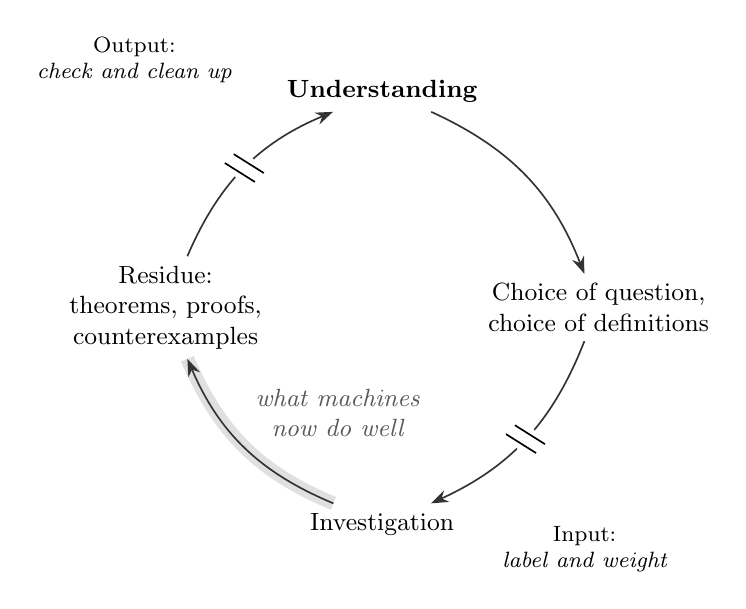
\begin{tikzpicture}[
    >={Stealth[length=2.2mm,width=1.6mm]},
    every node/.style={font=\small},
    lp/.style={->,semithick,black!80},
  ]
  \def\R{2.75}

  % -- the four moments of the loop --
  \node[align=center] (und) at ( 90:\R) {\bfseries Understanding};
  \node[align=center] (que) at (  0:\R) {Choice of question,\\choice of definitions};
  \node[align=center] (inv) at (270:\R) {Investigation};
  \node[align=center] (res) at (180:\R) {Residue:\\theorems, proofs,\\counterexamples};

  % -- the stretch the machines now cover --
  \draw[line width=5pt,black!12] (inv) to[bend left=22] (res);
  \node[align=center,font=\small\itshape,black!65] at (247:1.45)
       {what machines\\now do well};

  % -- the loop itself --
  \draw[lp] (und) to[bend left=22] (que);
  \draw[lp] (que) to[bend left=22] (inv);
  \draw[lp] (inv) to[bend left=22] (res);
  \draw[lp] (res) to[bend left=22] (und);

  % -- the two cuts, where the human meets the machine --
  \path (que) to[bend left=22] node[pos=.5,inner sep=0pt] (cutin)  {} (inv);
  \path (res) to[bend left=22] node[pos=.5,inner sep=0pt] (cutout) {} (und);
  \foreach \c/\a in {cutin/315, cutout/135}{%
    \begin{scope}[shift={(\c)},rotate=\a]
      \fill[white] (-0.24,-0.16) rectangle (0.24,0.16);
      \draw[semithick] (-0.22,-0.13) -- (0.22,-0.03);
      \draw[semithick] (-0.22, 0.03) -- (0.22, 0.13);
    \end{scope}}
  \node[align=center,font=\footnotesize\itshape] at (310:4)
       {\emph{Input:}\\label and weight};
  \node[align=center,font=\footnotesize\itshape] at (135:4.45)
       {\emph{Output:}\\check and clean up};
\end{tikzpicture}
\caption{\emph{The loop is the profession.} Understanding tells us where to look; looking is what produces understanding. Machines are now strong over one quarter of the circumference -- and not over the quarter that feeds it. The taste-labelling layer is this same loop cut at the two points where the human meets the machine.}
\label{fig:loop}
\end{figure}
% ---------------------------------------------------------------

\subsubsection{The open loop}


The ten problems of \S~\ref{sec:measure} are a live specimen of that cut, and of what falls through it. At the input, there is no co-author. There is a published narration of the model's reasoning, which one can read but not question: nobody to write to, nobody to invite to a seminar, nobody who can be asked why this direction and not another. A narration is a record of a path, not a partner on it.

At the output, the contribution to understanding is real but in its weakest form: what Thurston calls a collection of ``answers'', where what people wanted was understanding \cite[\S~1]{thurston1994}. The result is correct, documented -- and still to be converted. That conversion, which is reading, situating, exposing and teaching, is years of work; it is ours; and nothing in the announcement funds it. So the proofs are correct and \key{the loop is left open} -- and an open loop is not a slower loop, it is a different object.


\subsubsection{The loop kept whole: where to look}

The same loop, kept whole, points the other way. AI is \emph{a formidable trainer of intuition for reaching new research frontiers:} a doctoral student -- also any established researcher investigating outside their original field of expertise -- can test an intuition and build new understanding in afternoons where it used to cost months. Learning that one asked the wrong question was the most expensive lesson in a mathematical education; it is now nearly free.

What practice maintains, and a labelling layer cannot, is taste -- whose deep form, in fundamental mathematics, is the choosing of definitions (\S~\ref{sec:measure}).

\begin{pullquote}
  ``Knowning where to look'' is not a stock that can be harvested; it is maintained by practice. 
\end{pullquote}

Severed from practice, the layer degrades -- so the arrangement the fear imagines fails on its own terms.

\key{The danger is not the tool but the routing:} the next generation of researchers pushed toward the countable ends of the pipeline, because those are easy to fund and easy to measure -- and are precisely the parts that train no judgment.

Until now, nobody funded question-asking spontaneously; it produces nothing you can count. AI may change that: once the countable part costs nothing, the scarce part -- the question -- becomes visible, and acquires a value our socio-economic system never assigned it. \key{The bluff, called.}

\subsection{Compression is not acceleration}\label{sec:rate}

\keys{Rate problem\ksep proof abundance\ksep company time vs.\ generation time\ksep Thurston on foliations}

\subsubsection{From proof scarcity to proof abundance}

AI compresses the stages of the work that can be counted -- from an open problem to an argument on the page. It leaves untouched the stage that follows: the one in which a result is read, situated, exposed, taught, and eventually becomes part of what the field simply knows -- the closing of the loop\footnote{Researchers are now doing exactly this for one of OpenAI's ten solutions: turning the narration into scientific progress (see \cite{MO513866} and Footnote~\footref{ft:OAI3}).}. 

\begin{pullquote}
  Compressing the countable stages does not accelerate understanding; it widens the distance between what exists and what is understood.
\end{pullquote}

% ---------------------------------------------------------------
\begin{figure}[h]
\begin{minipage}[t]{0.33\linewidth}\small\itshape
  \vspace{0pt}
  \caption{\emph{Time compression of generation is not, by itself, acceleration of understanding} (schematic). One turn of the loop, from an open problem to a result one can build on. The angle is each stage's share of the turn; the radius is how long the turn takes, so nearer the centre is faster; the thicker the ring, the more broadly the understanding is held.}
  \label{fig:compression}
  \medskip
  Machines compress the early stages in every case alike -- but only where the closing stage is carried out does the turn shorten. Left open, it never closes at all: compression of the early stages alone cannot reach understanding.
\end{minipage}\hfill
\begin{minipage}[t]{0.63\linewidth}
\vspace{0pt}
\centering
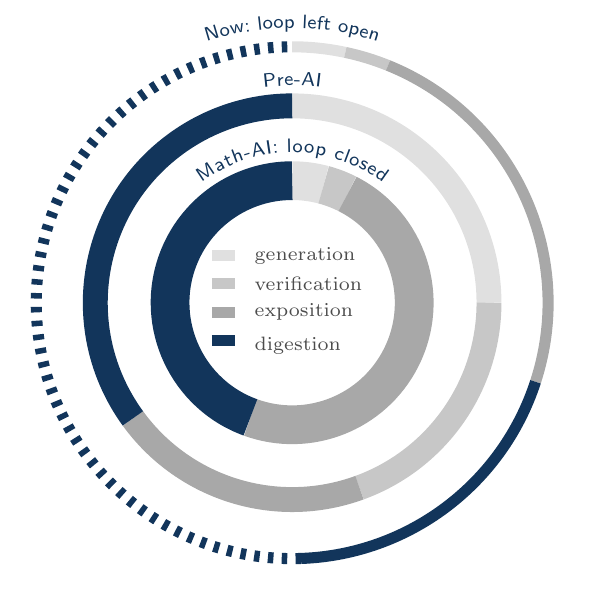
\begin{tikzpicture}[
    >={Stealth[length=2.0mm,width=1.5mm]},
    rC/.style={line width=14.0pt},   % Math-AI: loop closed
    rB/.style={line width=9pt},   % Pre-AI
    rO/.style={line width=4.0pt},   % Now: loop left open
    key/.style={font=\scriptsize,text=black!70,anchor=west},
  ]
  \def\Rc{1.55}   % Math-AI: loop closed -- fastest
  \def\Rb{2.50}   % Pre-AI
  \def\Ro{3.25}   % Now: loop left open

  % ---------- Math-AI: loop closed (inner) -- digestion 65% ----------
  \draw[rC,black!12] ( 90:\Rc) arc ( 90:  75:\Rc);   % generation    15
  \draw[rC,black!22] ( 75:\Rc) arc ( 75:  63:\Rc);   % verification  12
  \draw[rC,black!34] ( 63:\Rc) arc ( 63: -110:\Rc);   % exposition    99
  \draw[rC,Navy]     (-110:\Rc) arc (-110:-270:\Rc);   % digestion    234

  % ---------- Pre-AI (middle) -- digestion 35% ----------
  \draw[rB,black!12] ( 90:\Rb) arc ( 90:   0:\Rb);   % generation    90
  \draw[rB,black!22] (  0:\Rb) arc (  0: -70:\Rb);   % verification  70
  \draw[rB,black!34] (-70:\Rb) arc (-70:-144:\Rb);   % exposition    74
  \draw[rB,Navy]    (-144:\Rb) arc (-144:-270:\Rb);  % digestion    126

  % ---------- Now: loop left open (outer) -- digestion 70%, mostly undone ----------
  \draw[rO,black!12] ( 90:\Ro) arc ( 90:  78:\Ro);   % generation    12
  \draw[rO,black!22] ( 78:\Ro) arc ( 78:  68:\Ro);   % verification  10
  \draw[rO,black!34] ( 68:\Ro) arc ( 68: -18:\Ro);   % exposition    86
  \draw[rO,Navy]     (-18:\Ro) arc (-18: -88:\Ro);   % digestion done 70
  \draw[rO,Navy,dash pattern=on 2pt off 3pt]
                     (-88:\Ro) arc (-88:-270:\Ro);   % undone       182

  % ring labels, curved along each ring
  \path[decorate,decoration={text along path, text align={center}, raise=4.5pt,
        text={|\scriptsize\sffamily\color{Navy}|Math-AI: loop closed}}]
       (145:\Rc+0.20) arc (145:35:\Rc+0.20);
  \path[decorate,decoration={text along path, text align={center}, raise=2.5pt,
        text={|\scriptsize\sffamily\color{Navy}|Pre-AI}}]
       (145:\Rb+0.17) arc (145:35:\Rb+0.17);
  \path[decorate,decoration={text along path, text align={center}, raise=2.5pt,
        text={|\scriptsize\sffamily\color{Navy}|Now: loop left open}}]
       (145:\Ro+0.15) arc (145:35:\Ro+0.15);

  % ---------- key, in the eye of the rings ----------
  \begin{scope}[shift={(-1.02,0.60)}]
    \foreach \i/\c/\t in {0/black!12/generation, 1/black!22/verification,
                          2/black!34/exposition}
      {\draw[line width=4pt,\c] (0,-0.36*\i) -- (0.30,-0.36*\i);
       \node[key] at (0.42,-0.36*\i) {\t};}
    \draw[line width=4pt,Navy] (0,-1.08) -- (0.30,-1.08);
    \node[key,align=left] at (0.42,-1.15) {digestion};
  \end{scope}
\end{tikzpicture}
\end{minipage}
\end{figure}
% ---------------------------------------------------------------

A field can move faster and understand less, at the same time. Economists have a name for the missing quantity: \emph{absorptive capacity}, the ability to use knowledge produced elsewhere, built only by doing research oneself \cite{cohen1990} -- which is why free access to results confers little on a community that has stopped producing the people who can read and integrate them (\S~\ref{sec:structures}). 

Properly grounded, and held to the code of practice of the mathematical sciences (\S~\ref{sec:questions}), \emph{AI can however raise that capacity} -- the rate at which frontier work can be taken up -- by enhancing individual practice. The distinction matters: canonicalisation is slow because it requires broad deliberative consensus, and AI does not speed deliberation. What it can shorten is \emph{each participant's climb to the point of being able to take part.}

As Terence Tao (Fields Medal, 2006) states it plainly, if no ``suitable policy and cultural changes'' are made:

\begin{quotation}
[W]e will transition from an era of proof scarcity to an era of proof abundance.\\[0.2em]
\upshape\footnotesize\hfill -- T.~Tao \cite[slide 44]{icm2026}
\end{quotation}

Abundance is not, by itself, progress. The fact of a result travels cheaply; the horizon it opens does not. A thousand results nobody has travelled to will open little more than the fact of themselves.


\subsubsection{A mismatch of clocks}

Underneath is a mismatch of clocks. \key{Company time is release-cycle time; understanding takes root on the time of a generation.} The two cannot be brought into phase by working harder at the fast end -- which is the only end anyone is currently paying to speed up.


Nor is this a machine problem in origin. The precedent is at human scale and required no AI: Thurston's own account of his first subject, ``foliation theory'', where his flood of results emptied the field within a couple of years: colleagues were giving or receiving advice not to go into foliations -- they were saying that Thurston was cleaning it out'', and told him, not as a complaint, but as a compliment'', that he ``was killing the field''. He is explicit that the territory was not intellectually exhausted; what \emph{the rate of production destroyed were the \emph{ecological} conditions of the subject}, the ones under which anybody would want to keep thinking in it\endnote{Thurston's account, in \cite[\S~6]{thurston1994}, deserves quoting at length. Having ``fairly rapidly proved some dramatic theorems'' as a graduate student: \begin{quotation}\small\itshape An interesting phenomenon occurred. Within a couple of years, a dramatic evacuation of the field started to take place. I heard from a number of mathematicians that they were giving or receiving advice not to go into foliations -- they were saying that Thurston was cleaning it out. People told me (not as a complaint, but as a compliment) that I was killing the field. Graduate students stopped studying foliations, and fairly soon, I turned to other interests as well.\end{quotation} On the cause: ``I do not think that the evacuation occurred because the territory was intellectually exhausted -- there were (and still are) many interesting questions that remain and that are probably approachable.'' He names instead two ``ecological effects'': a high entry barrier, his results being ``documented in a conventional, formidable mathematician's style'' that ``depended heavily on readers who shared certain background and certain insights''; and the absence of anything left in it for anyone else -- ``More than the knowledge, people want personal understanding. And in our credit-driven system, they also want and need theorem-credits.'' 

The remedy he adopted afterwards is the one this section is arguing for: ``In reaction to my experience with foliations [\ldots] I concentrated most of my attention on developing and presenting the infrastructure'', publishing definitions and ways of thinking while remaining ``slow in stating or in publishing proofs of all the `theorems' I knew how to prove'', so as to ``[leave] room for many other people to pick up credit.''}. 

\key{A rate of production can destroy the conditions of understanding.} It is a rate problem before it is a machine problem -- and it now has a very much larger engine attached to it.


\subsection{The decision is ours}\label{sec:stake}

\keys{Priority vs.\ journey\ksep Library of Babel\ksep reproducibility\ksep authorship\ksep what cannot be mass-produced}

\subsubsection{Priority, and the journey}

A worry one hears from the next generation of researchers \cite{hampshire2026} has the shape of the Library of Babel -- Borges' library that contains every possible book, hence, somewhere on its shelves, every theorem, every proof, every refutation, already written. But this situation is already our condition: \emph{every researcher assumes that any result they obtain could be obtained by another trained mathematician.}

Is the experience of discovery being foreclosed? To answer, one must split ``discovery'' in two. One sense is priority -- first place in the world's ledger. That, machines will indeed make scarcer and noisier. The other is the journey -- the personal passage from confusion to understanding -- and it is indexed to a person, not to the ledger. 

\subsubsection{Nothing is lost}

The residue was always reproducible; \key{the journey never was.} Here the essayist quoted above puts it exactly right: ``human mathematics is Talmudic'' \cite{hampshire2026} -- the charge of learning comes from being conversant, across centuries, with the person who discovered. But then the conclusion inverts: if meaning travels through human authorship, the accumulated corpus -- the thing we spend our lives learning and teaching -- loses nothing to anything a machine proves afterwards. 

Each of us adds a little to a great deal that was already there: almost everything one will ever understand was discovered by someone else, and that has never once made the understanding less ours. For understanding is collective only in the way it is kept alive: not stored but re-walked -- each journey rebuilds a piece of the shared corpus in another mind\footnote{A philosophically inclined reader will recognise a Hegelian movement here: mathematical thought reaching a reflexive stage at which the \emph{Geist} recognises itself in its own productions -- transcending any particular individual, medium or epoch, while subsisting nowhere but in those who take it up again.}. 

That is why a machine's proof, which enters only the ledger, adds nothing to what the field actually understands: \key{the shared understanding lives only where someone has made the passage again.}

\subsubsection{What is actually at stake}

The machine takes nothing from what the field understands; it enlarges the residue and leaves the product untouched. What is genuinely at stake is not on the ledger at all -- and it is a decision, not a fate.

\begin{pullquote}
  The journey cannot be mass-produced -- and a collective understanding lives only where the journey is made. But it can be routed away, defunded, traded for what can be counted. That decision is ours, not the machine's.
\end{pullquote}

A decision of that kind shows itself in budget lines, in what a committee agrees to count, in the positions offered to people starting out -- and it is announced, plainly enough, in the collaborations struck with the new interface-structures (\S~\ref{sec:structures}).

The channel of discovery is not being sealed. It has become crowded and noisy -- not a bad problem to have, and one we already build for: curated libraries, large collaborative interfaces, machine-assisted formalisation.

{\itshape The journey, then, is not a private consolation; it is the piece the rest of this essay defends: what closes the loop (\S~\ref{sec:work}), what the rate endangers (\S~\ref{sec:rate}), and what the audit and the structures of \S~\ref{part:institutions} exist to keep funded.}

% ---------------------------------------------------------------
\begin{figure}[h]
\centering
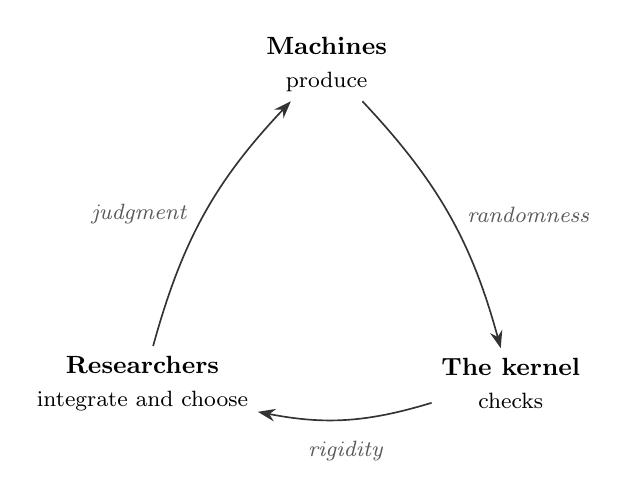
\begin{tikzpicture}[
    >={Stealth[length=2.2mm,width=1.6mm]},
    every node/.style={font=\small},
    lp/.style={->,semithick,black!80},
    lab/.style={font=\footnotesize\itshape,text=black!65},
  ]
  \def\R{2.7}

  % -- the three moments of the loop --
  \node[align=center] (mac) at ( 90:\R)
       {\bfseries Machines\\[0.1em]{\footnotesize produce}};
  \node[align=center] (ker) at (330:\R)
       {\bfseries The kernel\\[0.1em]{\footnotesize checks}};
  \node[align=center] (peo) at (210:\R)
       {\bfseries Researchers\\[0.1em]{\footnotesize integrate and choose}};

  % -- what each contributes, carried on the arcs --
  \draw[lp] (mac) to[bend left=14]
      node[lab,pos=.5,right=3pt,align=left]
      {randomness} (ker);
  \draw[lp] (ker) to[bend left=14]
      node[lab,pos=.5,below=4pt,align=center]
      {rigidity} (peo);
  \draw[lp] (peo) to[bend left=14]
      node[lab,pos=.5,left=3pt,align=right]
      {judgment} (mac);
\end{tikzpicture}
\caption{\emph{The virtuous loop.} People choose which questions are worth the asking; machines produce at a rate no community could sustain; the kernel makes what they produce checkable without its author having to be trusted, which opens the door to whoever's argument checks. Researchers integrate what arrives into the understanding -- and only that arc, the return to judgment, closes the loop.}
\label{fig:virtuous}
\end{figure}
% ---------------------------------------------------------------

\section*{Coda}

The models will keep producing mathematics, and mathematics will keep absorbing new modes of production, as it always has. The open questions do not belong to the machines: who checks, who trains, who pays -- and whether we continue to organise, and to fund, the one experience that was never reproducible in the first place.


\emph{A virtuous loop nonetheless becomes available:} machines propose at a rate no community could sustain; formalisation makes the proposals checkable without their authors having to be trusted; and, the material now being machine-tractable, \emph{the same tools can be turned back on it} -- questioned, replayed, explained -- so that expertise becomes something a newcomer builds rather than a barrier already cleared (Figure~\ref{fig:virtuous}). And once the corpus once grounded by researchers, those tools let far more of them read, question and answer one another than any seminar could hold. Read against Thurston's case, \emph{the virtuous loop lowers the entry cost of high-level knowledge for a more inclusive and diverse practice.}

None of that is automatic: it holds only where the practice is built for it. Such tools can be turned outward or inward: they can prepare more people to take part in a conversation, or they can answer in its place. \emph{Which happens is settled by the structures, not by the model.} The ``randomness'' from the LLMs, the ``rigidity'' from the kernel, and the judgment from people -- and the loop closes only on the third.

\begin{minipage}[t]{.45\linewidth}
  \vspace{0pt}
  \subsection*{Benjamin \textsc{Collas}}
  
  \medskip

  \small 
  Researcher at the Research Institute for Mathematical Sciences of Kyoto University (RIMS), working in arithmetic homotopy geometry -- a field that reconciles the rigidity of numbers with the flexibility of geometry. He leads the CNRS International Research Network \textsc{AHGT}, which links RIMS, the Universit\'e de Lille and the ENS-PSL, and brings together some $\sim$120 researchers in $\sim$15 countries.
  
  \medskip

  Email: \url{bcollas@kurims.kyoto-u.ac.jp}

  Web: \url{https://collas.perso.math.cnrs.fr}
\end{minipage}
\hfill
\begin{minipage}[t]{.45\linewidth}
  \vspace{0pt}
  \subsection*{Declaration on the use of AI}

  {\medskip \itshape
  The arguments, judgments and factual claims in this essay are the author's own. An AI assistant (Claude Fable~5 and Opus~4.8, Anthropic, accessed via Claude Code, July~2026) was used to draft and restructure English prose from the author's own writing and notes, for copy-editing, and editorial critique. 
  
  The author reviewed and revised all text, verified the sources, and takes full responsibility for the content.
  }  
\end{minipage}

{\addcontentsline{toc}{section}{Notes}
	\printendnotes
	}

% ===============================================================
\begin{thebibliography}{METI19}

  \bibitem[AMS24]{acadmathsci2024}
  Academy for the Mathematical Sciences, analysis of the economic contribution of the mathematical sciences in the UK, October 2024: \pounds495 billion of gross value added and 4.2 million people directly employed in mathematical science occupations (13\% of UK employment), on 2023 data. \url{https://www.acadmathsci.org.uk/publications/mathsci-supercharges-uk-econ-growth/}

  \bibitem[CNRS22]{CNRS22}
  CNRS, Institut national des sciences mathématiques et de leurs interactions (INSMI),
  \emph{Étude de l'impact économique des mathématiques en France}, 2022: 18\% of GDP and 3.3 million salaried jobs impacted by mathematics in France.


  \bibitem[Arr62]{arrow1962}
  K.~J. Arrow, \emph{Economic Welfare and the Allocation of Resources for Invention}, in \emph{The Rate and Direction of Inventive Activity: Economic and Social Factors}, NBER, Princeton University Press (1962), 609--626.

  \bibitem[CZC26]{CZC26}
  Ziyu Chen, Yilun Zhao, and Arman Cohan.
  \newblock {\em Measuring the Gap Between Human and LLM Research Ideas}.
  \newblock arXiv preprint arXiv:2607.01233, 2026.
  \newblock \url{https://arxiv.org/abs/2607.01233}.
  
  \bibitem[CL90]{cohen1990}
  W.~M. Cohen and D.~A. Levinthal, \emph{Absorptive Capacity: A New Perspective on Learning and Innovation}, Administrative Science Quarterly \textbf{35} (1990), 128--152.

  \bibitem[Del12]{deloitte2012}
  Deloitte, for the EPSRC and the Council for the Mathematical Sciences, \emph{Measuring the Economic Benefits of Mathematical Science Research in the UK}, June 2013: \pounds208 billion of gross value added (about 16\% of GVA) and 2.8 million jobs (about 10\% of employment), on 2010 data. Available from the London Mathematical Society, \url{https://www.lms.ac.uk/}

  \bibitem[EMS]{ems2012}
  European Mathematical Society, EMS Executive Committee, \emph{EMS Code of Practice for Mathematical Publication} (2025), on public claims of new theorems and timely provision of full details. \url{https://euromathsoc.org/code-of-practice}

  \bibitem[expM]{expmath}
  P.~Shafto (Rutgers University), \emph{expMath} (2025-28), a DARPA programme to accelerate the rate of progress in pure mathematics, \url{https://www.darpa.mil/research/programs/expmath-exponential-mathematics} 

  \bibitem[FFF26]{FFF26}
  Francesco Fournier-Facio,
  \emph{A torsion-free non-sofic group},
  Available at:
  \url{https://drive.google.com/file/d/1F1hBzrlGwX42z9hl0cd8SkosqlJcHYGt/view}
  (Accessed: 5 August 2026).

  \bibitem[FP26]{firstproof}
  First Proof, independent evaluation of AI systems on research-level mathematical problems under controlled conditions, with expert refereeing for correctness and exposition; seven of ten problems solved at publication-level quality, at \$10--\$1{,}000 of compute per problem. \url{https://1stproof.org} (2026).

  \bibitem[Goo75]{goodhart1975}
  C.~A.~E. Goodhart, \emph{Problems of Monetary Management: The U.K. Experience} (1975).
  
  \bibitem[Ham26]{hampshire2026}
  K.~Hampshire, \emph{The Dark Night of Mathematics -- What are we really doing?}, Substack, July 25, 2026. \url{https://kirwinhampshire.substack.com/p/the-dark-night-of-mathematics}

  \bibitem[ICM26]{icm2026}
  T.~Tao, \emph{Mathematics in the age of AI}, public lecture, International Congress of Mathematicians, 2026. \url{https://teorth.github.io/tao-web/slides/age-of-ai-icm-2026.pdf}

  \bibitem[Lei26]{leiden2026}
  J.~Portegies \emph{et al.} (working group of sixteen), \emph{Leiden Declaration on Artificial Intelligence and Mathematics}, June 2026. Drafted in the eight months following the conference \emph{Mechanization and Mathematical Research}, Lorentz Center, Leiden University, September 2025. DOI: \url{https://doi.org/10.5281/zenodo.20302944}.

  \bibitem[LS25]{LS25}
  D.~Loeffler and M.~Stoll, \emph{Formalizing zeta and L-functions in Lean}, Annals of Formalized Mathematics \textbf{1} (2025), 43--56. DOI: \url{https://doi.org/10.46298/afm.15328}.

  \bibitem[ML20]{ML20}
  The mathlib Community, \emph{The Lean Mathematical Library}, in Proc.~9th ACM SIGPLAN Int.~Conf.~on Certified Programs and Proofs (CPP 2020), 367--381. \url{https://arxiv.org/abs/1910.09336}

  \bibitem[METI19]{meti2019}
  Ministry of Economy, Trade and Industry and Ministry of Education, Culture, Sports, Science and Technology (Japan), \emph{The Coming Era of Mathematical Capitalism -- How the Power of Mathematics Changes Our Future} (Summary), Industry--Academia Round-Table Discussion, March 26, 2019.

  \bibitem[MO26]{MO513866}
  MathOverflow,
  ``What are the key new ideas in the proof of nonsoficity of groups in OpenAI's construction?''
  Question 513866,
  2026.
  \url{https://mathoverflow.net/questions/513866/what-are-the-key-new-ideas-in-the-proof-of-nonsoficity-of-groups-in-openai-s-con} (Accessed: 5 August 2026).

  \bibitem[Nel59]{nelson1959}
  R.~R. Nelson, \emph{The Simple Economics of Basic Scientific Research}, Journal of Political Economy \textbf{67} (1959), 297--306.

  \bibitem[OLS26]{OLS26}
  Parmy Olson,
  ``Math’s AI Crisis Has a Lesson For the Rest of Us,''
    \textit{Bloomberg Opinion}, forthcoming, Aug. 13, 2026.
    Available at: \url{https://www.bloomberg.com/opinion/articles/2026-08-13/math-faces-an-ai-spiritual-crisis-it-has-a-lesson-for-the-rest-of-us}.

  \bibitem[OAI26]{openai2026}
  OpenAI, \emph{Ten advances in mathematics and theoretical computer science}: announcement of solutions to ten long-open mathematical problems, 2026, \url{https://openai.com/index/ten-advances-in-mathematics/} 

  
  \bibitem[RHB26]{RHB26}
  A.~Freitas Ramos, D.~Barros Hulak, and
  R.~J.~Guerra Barretto de Queiroz.
  \newblock Formal Verification of an Explicit Counterexample to the Jacobian Conjecture.
  \newblock \emph{Archive of Formal Proofs}, July 2026.
  \newblock \url{https://isa-afp.org/entries/Jacobian_Counterexample.html},
  Formal proof development.

  
  \bibitem[Rom90]{romer1990}
  P.~M. Romer, \emph{Endogenous Technological Change}, Journal of Political Economy \textbf{98} (1990), S71--S102.

  \bibitem[SCH26]{SCH26}
  Eric Schmidt, ``The AI Revolution,'' Griswold Center for Economic Policy Studies
  Reunions Talk, Princeton University, moderated by Alan S. Blinder,
  May 22, 2026. Video: \url{https://www.youtube.com/watch?v=yS3rw9lPIPs}.

  \bibitem[SM01]{salter2001}
  A.~J. Salter and B.~R. Martin, \emph{The economic benefits of publicly funded basic research: a critical review}, Research Policy \textbf{30} (2001), 509--532.

  \bibitem[Thu94]{thurston1994}
  W.~P.~Thurston, \emph{On Proof and Progress in Mathematics}, Bulletin of the American Mathematical Society \textbf{30} (1994), 161--177.

  \bibitem[JCor75]{JCor75}
  C.~G.~J. Jacobi and A.-M. Legendre,
  \emph{Correspondance mathématique entre Legendre et Jacobi},
  Bulletin des sciences mathématiques et astronomiques,
  \textbf{9} (1875), 126--142.
  Available at: \url{https://www.numdam.org/item/BSMA_1875__9__126_1/}.

\end{thebibliography}


\vfill

\subsubsection*{\sffamily Version history}
\begin{itemize}
  \item 2026.08.13 - Bloomberg published; ArXiv submitted;
  \item 2026.08.05 - Additions: the investigation on non-sofic groups, Figure~\ref{fig:compression};
  \item 2026.08.01 - Version 1.
\end{itemize}
\end{document}
